\documentclass[12pt]{beamer}
\usepackage[utf8]{inputenc}
\usepackage[T1]{fontenc}
\usepackage[portuguese]{babel}
\usepackage{graphicx}
\usepackage{color}
\usepackage{slidesdef}

\title{Git - Introdução}
\author{Abel Siqueira}

\date{ 30 de Maio de 2015 }

\newcommand{\cmd}[1]{
\begin{flushleft}
{\color{yellow} \tt \$ #1 }\\
\end{flushleft}
}

\newcommand{\cmdinline}[1]{
{\color{yellow} \tt #1} }

\newcommand{\cmmt}[1]{
{\color{magenta} \tt \# #1} }

\newcommand{\bashgt}{ \textgreater\ }
\newcommand{\ddash}{-{}-}

\begin{document}

\myframe{
  \maketitle
}

\myframe{
  \ctr{Por quê?}

\begin{center}
  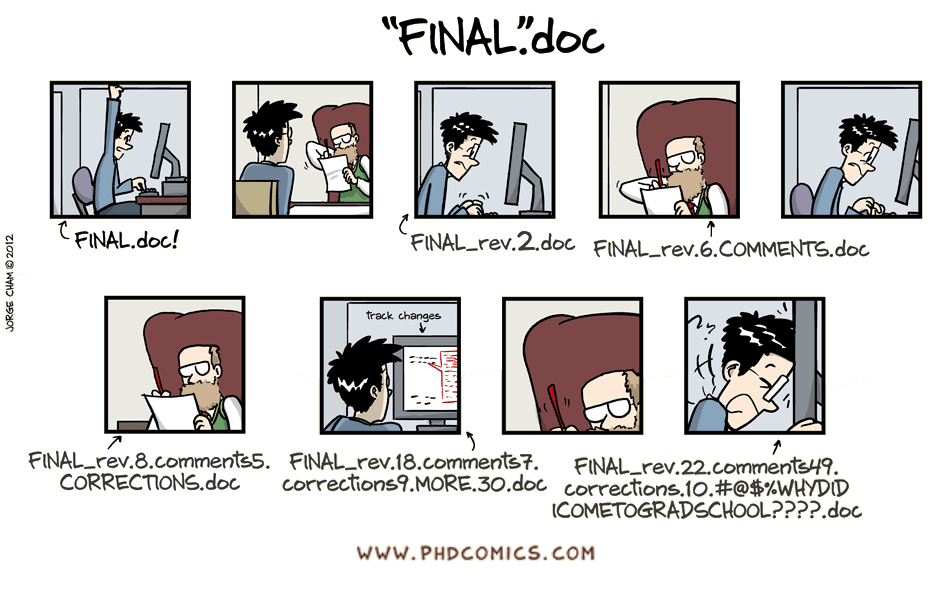
\includegraphics[height=0.8\textheight]{phd.png}
\end{center}
}

\myframe{
  \ctr{Como funciona?}
  \begin{center}
  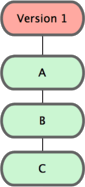
\includegraphics[height=0.5\textheight]{version1.png}
  \hspace{0.1cm}
  \pause
  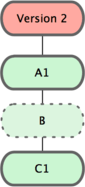
\includegraphics[height=0.5\textheight]{version2.png}
  \hspace{0.1cm}
  \pause
  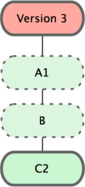
\includegraphics[height=0.5\textheight]{version3.png}
  \hspace{0.1cm}
  \pause
  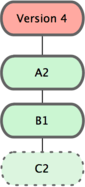
\includegraphics[height=0.5\textheight]{version4.png}
  \hspace{0.1cm}
  \pause
  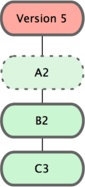
\includegraphics[height=0.5\textheight]{version5.png}
  \end{center}
}

\myframeblack{
  \ctrwhite{Começando}
  \begin{center}
    \tt \color{white}
    Uma vez na vida \onslide<2->{por computador}
  \end{center}
  \pause
  \pause
  \cmd{git config \ddash global user.name ``Seu nome''}
  \cmd{git config \ddash global user.email seu@email.com}
  \cmd{git config \ddash global color.ui auto}
}

\myframeblack{
  \ctrwhite{Começando}

  \cmd{mkdir aula-git}
  \cmd{cd aula-git}
  \cmd{git init}
  \cmd{ls -la}
  \pause
  \cmd{ls .git \only<3>{\cmmt{Não mexer}}}
}

\myframeblack{
  \ctrwhite{Criando e adicionando alguma coisa}

  \cmd{echo Meu noem eh Abel \bashgt teste}
  \pause
  \cmd{cat teste}
  \pause
  \cmd{git status}
  \pause
  \cmd{git add teste}
  \pause
  \cmd{git status}
}

\myframeblack{
  \ctrwhite{Primeiro commit}
  \cmd{git commit -m `Primeiro commit'}
  \pause
  \cmd{git status}
  \pause
  \cmd{git log}
}

\myframeblack{
  \ctrwhite{Modificando e adicionando mais arquivos}
  \cmd{\cmmt{Corrija teste (noem para nome)}}
  \cmd{cat teste}
  \pause
  \cmd{git status}
  \cmd{git diff}
  \pause
  \cmd{echo batata \bashgt compras}
  \cmd{git status}
}

\myframeblack{
  \ctrwhite{Modificando e adicionando mais arquivos}
  \cmd{git add teste}
  \pause
  \cmd{\cmmt{Mude eh para é em teste}}
  \pause
  \cmd{git status}
  \pause
  \cmd{git add compras}
  \cmd{git status}
  \pause
  \cmd{git commit -am `Segundo commit'}
  \cmd{\cmmt{-am é o mesmo que -a -m}}
  \pause
  \cmd{git log}
}

\myframe{
  \begin{center}
    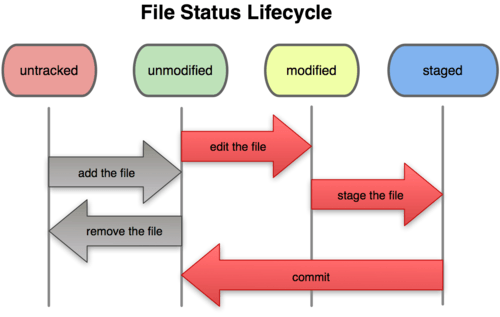
\includegraphics[width=0.95\textwidth]{status.png}
  \end{center}
}

\myframeblack{
  \ctr{\color{red} Já posso escrever meu código?}
  \pause
  \ctr{\color{green} SIM}
  \pause
  \ctr{\color{yellow} Mas espere. Tem mais.}
}

\myframeblack{
  \ctrwhite{Mensagens de commit}
  \cmd{echo ``\# Meu código'' \bashgt README.md}
  \cmd{git add README.md}
  \pause
  \cmd{git commit \cmmt{Sem -m}}
}

\myframeblack{
  \ctrwhite{Mensagens de commit}
  \begin{center}
  \begin{minipage}{0.9\textwidth}
    {\tt \color{green} Título (imperativo, 50-80 caracteres) \\ \\
      Texto da mensagem (70-100 caracteres por linha) \\
      Pode-se escrever a vontade, principalmente para explicar o motivo do
      commit.
    }
  \end{minipage}
  \end{center}
}

\myframeblack{
  \ctrwhite{Mensagens de commit}
  \tt \color{green}
  Faça o commit com o título ``Adiciona README.md'' e o texto ``README.md
  adicionado porque o Abel mandou''.
  \cmd{git log}
  \pause
  \cmd{git log \ddash oneline}
  \pause
  \cmd{git log \ddash graph}
  \cmd{git log \ddash graph \ddash oneline}
  \cmd{git log \ddash graph \ddash oneline \ddash decorate}
}

\myframeblack{
  \ctrwhite{Log bonito}
  \cmd{git log \ddash pretty=format:``\%ad (\%ar) \%n\%an
    (\%ae)\%n\%s\%n\%n\%b'' \ddash graph \ddash date=iso
  \onslide<2->{\cmmt{Vamos definir esse comando como meulog}}}
  \pause
  \pause
  \cmd{git config \ddash global alias.meulog `log \ddash pretty=format:``\%ad (\%ar)
    \%n\%an (\%ae)\%n\%s\%n\%n\%b'' \ddash graph \ddash date=iso'}
  \pause
  \cmd{git meulog}
}

\myframeblack{
  \ctrwhite{Help}
  \cmd{git help comando}
}

\myframecolor{gray!50!black}{
  \ctrwhite{Sumário}
  \cmd{git init}
  \cmd{git add}
  \cmd{git commit}
  \cmd{git status}
  \cmd{git log}
  \cmd{git diff}
  \cmd{git help}
}

\myframecolor{green!50!black}{
  \ctrcolor{green}{\Large Faça}
  \ctrcolor{white}{Commits frequentes}
  \ctrcolor{white}{Commits de assuntos relacionados}
  \ctrcolor{white}{Boas mensagens}
}

\myframecolor{red!50!black}{
  \ctrcolor{red}{\Large Não Faça}
  \ctrcolor{white}{Commits monolíticos}
  \ctrcolor{white}{Inclusão de arquivos que são gerados (facilmente)}
  \ctrcolor{white}{Commits sem testar o trabalho}
}

\myframe{
  \ctr{\Huge Fim\onslide<2->{?}}
}

\usetikzlibrary{trees}

\tikzset{
  commit/.style = {draw, circle},
  invisible/.style={opacity=0},
  visible on/.style={alt=#1{}{invisible}},
  alt/.code args={<#1>#2#3}{
    \alt<#1>{\pgfkeysalso{#2}}{\pgfkeysalso{#3}}
  }
}

\newcommand{\gitcommit}[1]{ node[commit] (#1) {#1} }
\newcommand{\gitref}[2]{ \draw (#1) -- +(0,0.7) node[above] (#2) {#2}; }
\newcommand{\gitrefd}[2]{ \draw (#1) -- +(0,-0.7) node[below] (#2) {#2}; }

\myframeblack{
  \begin{center}
  \begin{tikzpicture}[grow via three points={one child at (1.5,0) and two children
      at (1.5,0) and (1.5,-1.5)}, <-, white]
    \node[commit] (C1) {C1}
    child[visible on=<2->]{
      \gitcommit{C2}
      child[visible on=<3->]{
        \gitcommit{C3}
        child[visible on=<4->]{
          \gitcommit{C4}
          child[visible on=<10->]{
            \gitcommit{C7}
            child[visible on=<11>]{
              \gitcommit{C8}
            }
          }
        }
      }
      child[visible on=<7->]{
        \gitcommit{C5}
        child[visible on=<8->]{
          \gitcommit{C6}
        }
      }
    }
    ;
    \onslide<1>{\gitref{C1}{master}\gitref{master}{HEAD}}
    \onslide<2>{\gitref{C2}{master}\gitref{master}{HEAD}}
    \onslide<3>{\gitref{C3}{master}\gitref{master}{HEAD}}
    \onslide<4>{\gitref{C4}{master}\gitref{master}{HEAD}}
    \onslide<5-8>{\gitref{C4}{master}}
    \onslide<5>{\gitref{C2}{HEAD}}
    \onslide<6>{\gitref{C2}{issue}\gitref{issue}{HEAD}}
    \onslide<7>{\gitrefd{C5}{issue}\gitrefd{issue}{HEAD}}
    \onslide<8>{\gitrefd{C6}{issue}\gitrefd{issue}{HEAD}}
    \onslide<9-11>{\gitrefd{C6}{issue}}
    \onslide<9>{\gitref{C4}{master}\gitref{master}{HEAD}}
    \onslide<10>{\gitref{C7}{master}\gitref{master}{HEAD}}
    \onslide<11>{\gitref{C8}{master}\gitref{master}{HEAD}}
    \onslide<11>{ \draw (C6) -- (C8); }
  \end{tikzpicture}
  \end{center}

  \only<1-4>{ \cmd{git commit} }
  \only<5>{ \cmd{git checkout C2} }
  \only<6>{ \cmd{git branch issue} }
  \only<7-8>{ \cmd{git commit} }
  \only<9>{ \cmd{git checkout master} }
  \only<10>{ \cmd{git commit} }
  \only<11>{ \cmd{git merge issue} }
}

\myframecolor{gray!50!black}{
  \ctrwhite{Sumário 2}
  \cmd{git branch}
  \cmd{git checkout}
  \cmd{git merge}
}

\myframe{
  \ctr{\Huge Fim}
}

\end{document}
